
\title{The Four Fundamental Subspaces}
\subtitle{\SubTitleName}
\institute[]{\Course}
\author{\Instructor}
\maketitle   
  

\frame{\frametitle{Topics and Objectives}
\Emph{Topics} \\
%\TopicStatement
\begin{itemize}

    % \item dot products

    % \item magnitude of vectors
    
    % \item distances in $\mathbb R^n$ 
    
    % \item angles between vectors

    \item relationships between $\Row A$, $\Col A$, $\Nul A$, and $\Nul A^T$
    

\end{itemize}

\vspace{0.5cm}

\Emph{Learning Objectives}\\

\LearningObjectiveStatement

\begin{itemize}

    \item construct a basis for the four fundamental subspaces of a rectangular matrix
    
\end{itemize}

} 


\begin{frame}\frametitle{Row$A$}
    
    \begin{center}
    \begin{tikzpicture} \node [mybox](box){\begin{minipage}{0.75\textwidth}
        \vspace{2pt}
        
        Row$A$ is the space spanned by the rows of matrix $A$.

        \end{minipage}};\node[fancytitle, right=10pt] at (box.north west) {Definition};
    \end{tikzpicture}
    \end{center}

	We can show that
	\vspace{6pt}
	\begin{itemize} \setlength\itemsep{1em}
		\item<2-> a basis for Row$A$ is given by the pivot rows of $A$
		\item<3-> $\dim(\Row A) = \dim(\Col A)$
	    \item<4-> $\Row A = \Col A^T$
	    \item<5-> in general $\Row A$ and $\Col A$ are not related to each other
	\end{itemize}

\end{frame}









\begin{frame}{Revisiting the Rank Theorem}

    Recall from earlier in the course, that if $N$ is the number of columns in a matrix, that
    
    $$N = \dim (\Col A) + \dim (\Nul A)$$
    \vspace{2pt}
    \pause
    
    But if dim(Row $A$) = dim(Col $A$), then we could express this as
    
    $$N = \dim (\Row A) + \dim (\Nul A)$$
    \vspace{2pt}
    \pause
    
    In fact, there are many other equivalent ways of expressing the above theorem. 
    
\end{frame}



\begin{frame} \frametitle{Relationships Between $\Row A$ and $\Nul A$} 

    % Describe the Null$(A)$ in terms of an orthogonal subspace.  \\[12pt]
    
    Suppose vector $ \vec v$ is in $ \Null A$.
    
    \vspace{4pt}

    \begin{itemize}  \setlength\itemsep{1em}
    
        \item<1-> then $ A \vec v =  \vec 0$
        
        \item<2-> we compute $A\vec v$ by taking dot products between each row of $A$ and $\vec v$
        
        \item<3-> all of these dot products are zero, so $ \vec v$ is orthogonal to the rows of $A$

        \item<4-> therefore, $\Row A  $ is  orthogonal to $\Null A $
        
        \item<5-> in other words, $(\Row A)\Perp = \Null A$

    \end{itemize}
    
    \vspace{4pt}
    \onslide<6->{Or, we could also say that $\Row A = (\Null A)\Perp$. }
    
\end{frame}


\begin{frame} \frametitle{Relationships Between Col$A$ and Nul$A^T$} 

    There is a similar relationship between $\Col A$ and $\Nul A^T$. Suppose vector $ \vec x$ is in $ \Null A^T$.

    \begin{itemize}  \setlength\itemsep{1em}
        \item<1-> then $ A^T \vec x =  \vec 0$
        
        \item<2-> this implies that $ \vec x$ is orthogonal to the rows of $ A^T$

        \item<3-> this implies that $ \vec x$ is orthogonal to the columns of $ A$

        \item<4-> therefore, $\Col A  $ is  orthogonal to $\Null A^T $
        
        \item<5-> in other words, $(\Col A)\Perp = \Nul A^T$

    \end{itemize}
    
    
\end{frame}




\begin{frame}{The Four Fundamental Subspaces}

    \begin{center}\begin{tikzpicture} \node [mybox](box){\begin{minipage}{0.85\textwidth}\vspace{2pt}
    For any $ A \in \mathbb R^{m\times n}$,  the orthogonal complement of $\Row A$ is $ \Null A$, and the orthogonal complement of $ \Col A$ is  $ \Null A ^{T}$.  

    \end{minipage}};
    \node[fancytitle, right=10pt] at (box.north west) {Theorem (The Four Subspaces)};
    \end{tikzpicture}\end{center}

    % The idea behind this theorem is described in the diagram below. 
    \pause 
    
    \begin{center}
    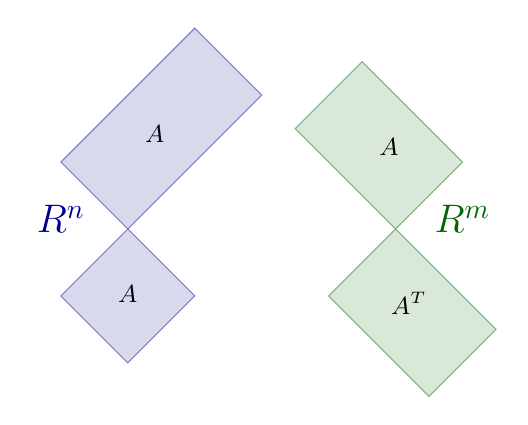
\begin{tikzpicture}[scale=.85]
        

        
        \onslide<2->{
        % boxes
        \filldraw[draw=DarkBlue!50,fill=DarkBlue!15] (0,0) -- (-1,1) -- (1,3) -- (2,2) -- cycle;
        \filldraw[draw=DarkBlue!50,fill=DarkBlue!15] (0,0) -- (1,-1) -- (0,-2) -- (-1,-1) -- cycle;      
        \draw (0.4, 1.7) node[below]{\small $\Row A$};
        \draw (0.0,-0.7) node[below]{\small $\Nul A$};        
        }
        
        \onslide<3->
        {
        \filldraw[draw=DarkGreen!50,fill=DarkGreen!15] (4,0) -- (2.5, 1.5) -- (3.5, 2.5) -- (5,1) -- cycle;
        \filldraw[draw=DarkGreen!50,fill=DarkGreen!15] (4,0) -- (5.5,-1.5) -- (4.5,-2.5) -- (3,-1) -- cycle;        
        \draw (3.9, 1.5) node[below]{\small $\Col A$};
        \draw (4.2, -0.8) node[below]{\small $\Nul A^T$};        
        }

        \onslide<4->{
        \draw (-1.0,0.5) node[below]{\Large $\color{DarkBlue} \mathbb R^n$};
        }

        \onslide<5->{
        \draw ( 5.0,0.5) node[below]{\Large $\color{DarkGreen} \mathbb R^m$};
        }
        
    \end{tikzpicture}
    \end{center}

\end{frame}

\begin{frame}\frametitle{Example} 

    Suppose $A = \spalignmat{1 3 0 ; 0 0 1 ; 0 0 0 }$. Construct a basis for the following.
    \begin{enumerate} \setlength{\itemsep}{24pt}
        \item $\Row A$
        \item $(\Row A)^{\perp}$
        \item $\Col A$
        \item $(\Col A)^{\perp}$    
    \end{enumerate}

\end{frame}



\frame{\frametitle{Summary}

    \SummaryLine \vspace{4pt}
    \begin{itemize}\setlength{\itemsep}{8pt}

    \item orthogonality relationships between the four fundamental subspaces: $\Row A, \Col A, (\Row A)\Perp,$ and $(\Col A)\Perp$
    
    \end{itemize}
    
    \vspace{8pt}
    
}







% \begin{frame}\frametitle{Additional Example (if time permits)}
%     $A$ has the LU factorization: 
        
%         $$A=L U = \spalignmat{1 0 0;1 1 0;0 4 1} \spalignmat{1 0 2 0;0 1 -1 2;0 0 0 0}$$
        
%         \begin{itemize}[a)]
%             \item Construct a basis for $(\mathrm{Row}A)^{\perp}$
%             \item Construct a basis for $(\mathrm{Col}A)^{\perp}$
%         \end{itemize}
%         \textit{Hint: it is not necessary to compute $A$. Recall that $A^T = U^TL^T$, matrix $L^T$ is invertible, and $U^T$ has a non-trivial nullspace}. 
% \end{frame}




% \begin{frame}\frametitle{Looking Ahead - Projections}

%     Suppose we want to find the closest vector in Span$\{\vec b\}$ to $\vec a$. 
%      \begin{center}
%         \begin{tikzpicture}[scale=0.8] 
%             \draw[-,gray, dashed] (-1,-1/9) -- (11,11/9) node[below, right] {Span$\{\vec b\}$}; 
%             \draw[->,DarkBlue, thick,-stealth] (0,0) -- (9,1) node[below,right] {$ \vec b$}; 
%             \draw[->,DarkRed, thick,-stealth] (0,0) -- (3,3) node[above] {$ \vec a = \hat a + \vec w$}; 
%             \draw[->,black, very thick,-stealth] (0,0) -- (3.3,3.3/9) node[below] {$\hat a = $proj$_{\vec b} \vec a$}; 
%             \draw[->,DarkGreen,very thick, dashed, -stealth] (3.3,3.3/9) -- (3,2.8) node[below, right] {$\vec w$}; 
%             %\draw[black] (2,2/9) arc (0:100:0.85) node[midway, right] {$\theta$};            
%         \end{tikzpicture}
%     \end{center} 
    
%     \begin{itemize}
%         \item later we draw connections between dot products and \Emph{projections}
%         % \item the 
%         \item projections are also used throughout multivariable calculus courses
%     \end{itemize}    
    
% \end{frame}
 



